\documentclass[11pt,a4paper]{article}

\usepackage[T1]{fontenc}
\usepackage[utf8]{inputenc}
\usepackage{newtxtext,newtxmath}   % Times-like text and math
\usepackage{microtype}
\usepackage{graphicx}
\usepackage{booktabs}
\usepackage{tabularx}
\usepackage{amsmath}
\usepackage[ruled,vlined,linesnumbered]{algorithm2e}
\usepackage[numbers,sort&compress]{natbib}
\usepackage{xcolor}
\usepackage{geometry}
\geometry{a4paper, top=2.6cm, bottom=2.6cm, left=2.6cm, right=2.6cm}

\definecolor{linkblue}{HTML}{1a4a7a}
\usepackage[colorlinks=true, linkcolor=linkblue, citecolor=linkblue,
            urlcolor=linkblue, bookmarks=true]{hyperref}

\widowpenalty=10000
\clubpenalty=10000

\hypersetup{
  pdftitle={Wet-Ink: Sliding-Window Frontier Decoding for Diffusion Language Models},
  pdfauthor={Ozodbek Asilbekov},
  pdfsubject={Diffusion language models; decoding strategies; inference-time token revision},
  pdfkeywords={diffusion language models, decoding, token editing, LLaDA, wet-ink}
}

\setlength{\parskip}{0pt}

\begin{document}

% ===================== Title block =====================
\begin{center}
  {\LARGE\bfseries Wet-Ink: Sliding-Window Frontier Decoding\\[0.35em]
  for Diffusion Language Models\par}
  \vspace{1.4em}
  {\large Ozodbek Asilbekov\par}
  \vspace{0.35em}
  {\normalsize Independent Researcher (Freedomform)\par}
  \vspace{0.35em}
  {\small November 2026\par}
\end{center}

\vspace{0.9em}
\noindent\rule{\textwidth}{0.5pt}
\vspace{0.4em}

\begin{center}\begin{minipage}{0.9\textwidth}
\textbf{Abstract.}
Diffusion language models (dLLMs) generate tokens with parallel denoising passes over
blocks of masks, and every published block decoder commits a whole block before moving on:
once a block closes, its tokens are frozen. We study \emph{wet-ink decoding}, an
inference-time schedule in which a diffusion \emph{frontier} opens tokens strictly
left-to-right, exactly one per denoising step, while a \emph{sliding window} of $W$
tokens behind the frontier remains revisable through the base model's own trained
token-to-token (T2T) editing gate; at distance $W$ the ink \emph{dries} and a token is
never touched again. The method is implemented on LLaDA2.2-mini
(16B MoE, 1.4B active) under a strict zero-invention policy: every mechanism~--- the
greedy frontier commit, the trained gate $p_0>\tau_e \wedge x_i \neq x_0$, SPLIT/DELETE
edit operations, the anti-loop resampler, and block-diagonal attention~--- is reused
verbatim from the base model, and the decoding schedule is the only new variable, which
block-diffusion theory identifies as a legitimate free inference-time choice.
On GSM8K under a paired exact protocol (identical model, 4-bit quantization, prompts,
and task indices), wet-ink decoding matches the stock parallel decoder on every arm:
11/45 versus 11/45 against the stock baseline (McNemar $p=1.0$) and zero outcome flips
against a frontier-only control across 22 common tasks, although the editing gate fires
6.9 times per task. The apparent $+10.8$-point accuracy gap over the internal control is
a task-composition artifact, which we expose with a segment analysis. The cost is
structural: $\times 4.88$ network-function evaluations. We report this as a controlled
negative result, the third consecutive one in our five-version program, and discuss what
it implies for inference-time token revision in diffusion language models.
\end{minipage}\end{center}

\vspace{0.4em}
\noindent\rule{\textwidth}{0.5pt}
\vspace{0.8em}

% ===================== 1. Introduction =====================
\section{Introduction}\label{sec:intro}

Autoregressive language models commit each token exactly once, in a fixed left-to-right
order. Diffusion language models (dLLMs) relax both constraints: they denoise all
positions of a block in parallel and may rewrite any still-masked position at any step
\citep{llada,dream7b,llada22mini}. The relaxation buys parallelism and controllability
but discards a property that writers of prose take for granted: the ability to
\emph{commit} early text while keeping a bounded amount of recent text correctable. A
human writer does not re-plan the first sentence of every paragraph; nor do they freeze
each word the instant it is written. The leading edge of the text is wet; old ink dries.

We call the decoding schedule that formalizes this intuition \emph{wet-ink decoding}
(Figure~\ref{fig:method}). A one-token \emph{frontier} opens the leftmost remaining
mask at every denoising step, committing it autoregressively; a \emph{wet window} of
$W$ positions behind the frontier stays revisable; at distance $W$ there is a
\emph{hard dry edge} beyond which tokens are frozen forever. The frontier is the
one-token-per-step end of the published autoregression--diffusion interpolation
spectrum \citep{bd3lm,setdiffusion}; the wet window is realized not by a new
confidence heuristic but by the base model's own \emph{trained} T2T editing gate from
LLaDA2.2's Levenshtein editing machinery \citep{llada22mini,llada21}, windowed in time.

Two design commitments distinguish this work from prior attempts at token revision in
dLLMs. First, a \emph{zero-invention policy}: no new formulas and no modifications of
published ones; every primitive is taken verbatim from the base model's code, with
line-level provenance, and the only new object is the schedule that orders the
application of these primitives. Block diffusion theory makes this position precise:
tokens-per-step and position orderings are free inference-time variables, not model
changes \citep{bd3lm,setdiffusion}. Second, an \emph{adversarial evaluation protocol}:
paired task indices, exact McNemar tests, Wilson intervals, and network-function-evaluation
(NFE) accounting on every arm, so that neither task sampling nor compute asymmetries
can masquerade as an effect.

The empirical outcome is unambiguous and, we argue, worth publishing as such. On GSM8K
with LLaDA2.2-mini, wet-ink decoding is \emph{pair-identical} to the stock parallel
decoder: against the stock baseline the score is 11/45 versus 11/45 (2 outcomes fixed,
2 broken, exact McNemar $p=1.0$); against a frontier-only control that disables window
editing, not a single one of 22 common tasks flips, although the trained gate genuinely
fires 6.9 times per task. The price is structural: $\times 4.88$ NFE, because committing
one token per step forfeits the parallelism of block decoding. A visible $+10.8$-point
raw gap over the internal control turns out to be a task-composition artifact~--- the
control arm stopped early on the hardest segment of the benchmark~--- which we
demonstrate explicitly (Section~\ref{sec:artifact}).

This paper is the fifth iteration of a research program that treats the wet-ink idea as
a hypothesis to be attacked rather than demonstrated. Versions 1--3 tested
training-free revision rules on Nemotron-Labs-Diffusion-3B and found them neutral to
harmful; version 4 audited the stock decoding parameters of LLaDA2.2-mini; version 5,
reported here, is the first implementation of the idea as an actual decoder
(Section~\ref{sec:journey}). The program thus yields three independent, paired,
consistently null results on the same hypothesis family, which is exactly the evidence
the community currently lacks about inference-time token revision in dLLMs
\citep{remeval}.

Our contributions are:
\begin{itemize}\itemsep2pt
  \item \textbf{A wet-ink decoder} for LLaDA2.2-mini: a one-token left-to-right
        frontier with a sliding window of $W$ revisable tokens, a hard dry edge, built
        exclusively from the base model's own trained mechanisms under a
        zero-invention policy with full provenance.
  \item \textbf{A paired evaluation protocol} for decoding schedules: exact McNemar
        tests on common task indices, Wilson intervals, NFE accounting, and
        task-composition controls.
  \item \textbf{A controlled negative result}: the trained editing gate, given a
        sliding window and an honest budget, does not move task accuracy on GSM8K ---
        with a segment-level analysis showing why raw gaps in small-$n$ benchmark runs
        can be pure composition artifacts.
\end{itemize}

\begin{figure}[t]
  \centering
  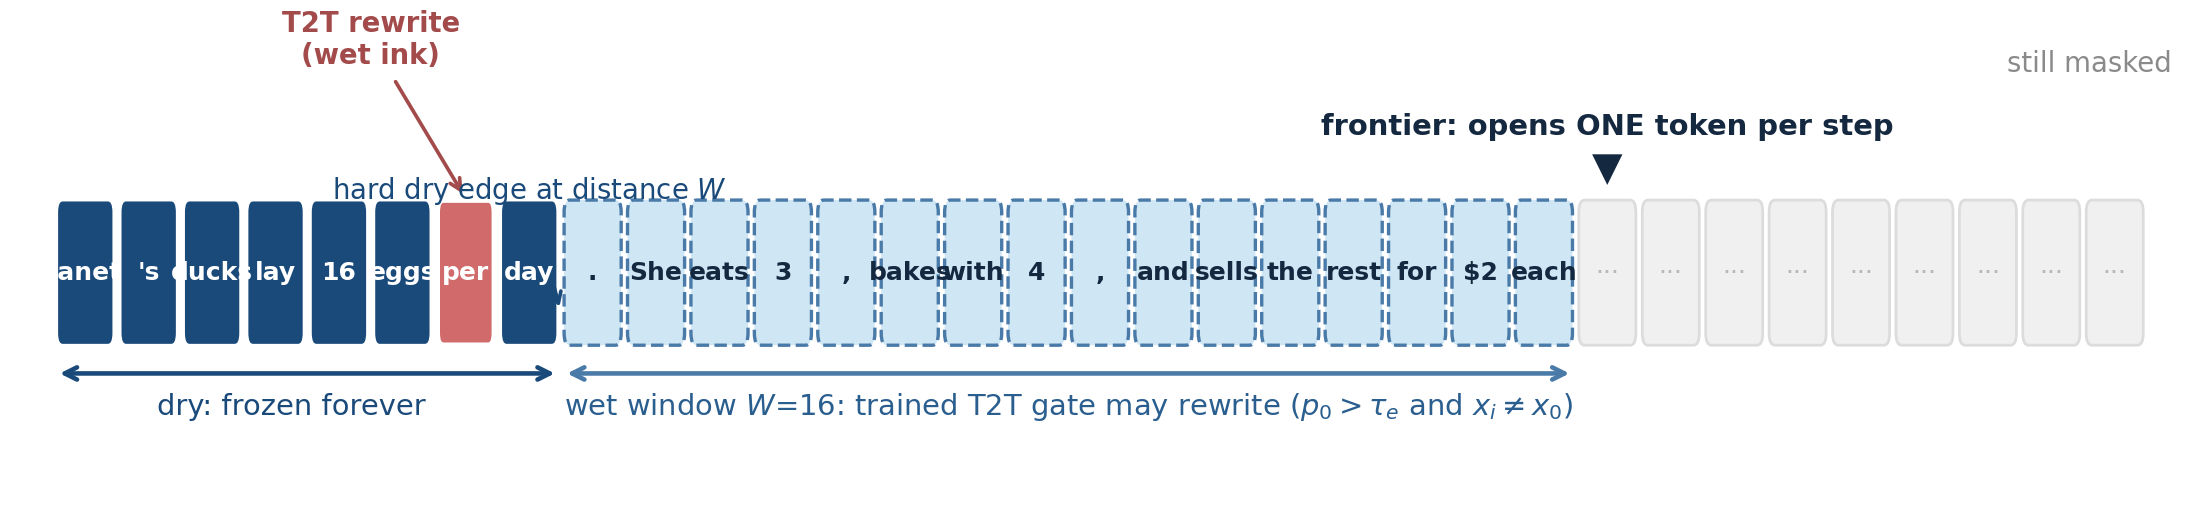
\includegraphics[width=\textwidth]{fig_method.png}
  \caption{\textbf{Wet-ink decoding.} Each denoising step commits exactly one token at
  the frontier (left-to-right). A sliding window of $W{=}16$ positions behind the
  frontier stays revisable through the model's trained T2T gate (one rewrite shown in
  red); positions farther from the frontier are dry and are never touched again.}
  \label{fig:method}
\end{figure}

% ===================== 2. Background and Related Work =====================
\section{Background and Related Work}\label{sec:background}

\subsection{Masked diffusion language models and block decoding}
Masked dLLMs such as LLaDA \citep{llada} and Dream 7B \citep{dream7b} generate by
iteratively denoising a span of \texttt{[MASK]} tokens. The standard inference
implementation is \emph{block decoding}: the response of length $L$ is split into
blocks of $B$ tokens (typically $B{=}32$); within a block, each denoising step
predicts all positions at once, a transfer schedule allocates how many tokens each
step may commit, a confidence threshold governs which candidates are accepted, and
once the block's masks are resolved the block is frozen forever~--- its tokens are
never revisited. LLaDA2.2-mini \citep{llada22mini} augments this pipeline with
\emph{Levenshtein editing} \citep{llada21,levt}: trained \texttt{DELETE} and
\texttt{SPLIT} operations, an anti-loop resampler, and a token-to-token (T2T)
editing gate that may replace a previously opened token with a new prediction when
the model is confident and the prediction differs. The editing window of the stock
implementation is the \emph{current block only}: when a block closes, its ink dries
at once, and no later block can repair it. Our starting question was whether a
window that \emph{slides} behind a moving frontier~--- wet ink that dries gradually
rather than blockwise~--- changes anything.

\subsection{The autoregression--diffusion interpolation spectrum}
That the ordering and granularity of token commits are free inference-time
variables, not model properties, is the central insight of the block-diffusion
line of work. BD3-LM \citep{bd3lm} trains block-AR discrete diffusion models in
which block sizes trade parallelism against conditioning; Set Diffusion
\citep{setdiffusion} goes further and interpolates \emph{token orderings} between
fully parallel (diffusion) and fully left-to-right (autoregressive) decoding at
inference time, reporting favorable speed--quality trade-offs. Our frontier~--- one
token per step, strictly left-to-right~--- is exactly the autoregressive end of
this spectrum, composed with the stock denoising machinery of a fixed trained
model. Related efficiency work optimizes the sampling schedule \citep{jys},
decodes adaptively in parallel \citep{apd}, or caches attention across steps
\citep{fastdllm}; all are orthogonal to token revisability, which is our subject.

\subsection{Token revision and remasking}
Revising opened tokens is a recognized open problem. RemeDi \citep{remedi}
\emph{trains} a remask-aware model whose per-token confidence decides which open
tokens to re-mask each step; its inference code re-masks cumulatively top-$k$
scored positions. A family of \emph{training-free} rules adapts the same idea to
fixed models: WINO, Saber \citep{saber}, and COVER re-mask low-confidence open
tokens under various budgets; CoDR \citep{codr} masks a partition of the window,
measures the confidence drift of the remaining tokens, and re-masks on drift.
Self-correcting masked diffusion \citep{proseco} learns a corrector module.
The recent calibration study of \citet{remeval} is the most direct precedent for
our skepticism: under greedy decoding and short blocks, all three training-free
remasking rules they test perform on par with confidence-based unmasking alone,
and their analyses locate the bottleneck in the dLLM itself, suggesting that
effective revision may require changes to \emph{training}, not merely to inference.

Our program engaged this literature sequentially before building the v5 decoder
reported here: v2--v3 ported RemeDi's and CoDR's published cycles verbatim to
Nemotron-Labs-Diffusion-3B and found them neutral (CoDR) to significantly harmful
(RemeDi, $-19.5$ to $-31.5$ points on GSM8K/HumanEval, $p<0.001$), exactly the
flip-flop behavior predicted by \citet{remeval}; v4 audited the stock editing
parameters of LLaDA2.2-mini; v5 finally gave the trained editing gate the sliding
window it never had. The full lineage is summarized in Section~\ref{sec:journey}.

% ===================== 3. Method =====================
\section{The Wet-Ink Decoder}\label{sec:method}

\subsection{Stock block decoding of LLaDA2.2-mini}
Let $x \in \mathcal{V}^{B}$ be the current block of $B$ positions, some of them
open (decoded) and some \texttt{[MASK]}ed. One stock denoising step computes, for
every position $i$, a categorical $p(\cdot \mid x)$ over the vocabulary, the greedy
prediction $x_0(i) = \arg\max_v p(v \mid x)$, and its confidence
$p_0(i) = p\!\left(x_0(i) \mid x\right)$. A per-step token budget
$n_t$ (the even-split \emph{transfer schedule} with the remainder assigned to
early steps) determines how many masks may open: candidates are ranked by
confidence, and a mask opens if it is within the budget and its confidence exceeds
the threshold $\tau$. After all masks of the block are resolved, a post-phase of up
to $S$ further steps may \emph{edit} open tokens of the same block through the
trained T2T gate
\begin{equation}\label{eq:t2t}
\mathrm{edit}(i) \;=\; \mathbb{1}\!\left[\, p_0(i) > \tau_e \,\wedge\, x_i \neq x_0(i) \,\right],
\end{equation}
combined with trained \texttt{SPLIT}/\texttt{DELETE} operations, an anti-loop
resampler, and residual special-token suppression; then the block freezes forever.
Attention within the block uses the model's block-diagonal mask; blocks attend to
all previous (frozen) blocks causally. Editing is thus confined to the current
block: there is no mechanism, in any configuration of the stock parameters, for a
later block to repair an earlier one.

\subsection{The wet-ink schedule}
Wet-ink decoding keeps every one of these primitives and changes only the
schedule: which position opens, and which positions stay revisable, at each step.

\paragraph{Frontier.}
Within the current block, define the frontier $f$ as the number of leading
positions already committed. Each denoising step opens \emph{exactly one} token ---
the leftmost remaining mask~--- and commits it greedily
($T{=}0$, deterministic):
\begin{equation}\label{eq:frontier}
x_f \leftarrow x_0(f), \qquad f \leftarrow f + 1 .
\end{equation}
Progress is guaranteed by construction: each step removes exactly one mask, so the
block resolves in exactly $B$ steps~--- no step limit is ever reached, and the
churn explosions of our v1 (Section~\ref{sec:journey}) cannot occur. This is the
one-token-per-step, left-to-right end of the ordering spectrum of
\citet{setdiffusion}.

\paragraph{Wet window and hard dry edge.}
Behind the frontier, the $W$ most recent positions stay revisable through the
stock gate of Equation~\eqref{eq:t2t}. Formally, we override the model's editing
confidence field with a windowed version,
\begin{equation}\label{eq:window}
\tilde{p}_0(i) \;=\;
\begin{cases}
p_0(i), & f - W \leq i < f \quad \text{(wet)}\\[2pt]
-\infty, & \text{otherwise} \quad \text{(dry)}
\end{cases}
\end{equation}
and run the unmodified gate $\mathbb{1}[\tilde{p}_0(i) > \tau_e \wedge x_i \neq
x_0(i)]$. The window is clipped to the current block, matching the model's
block-diagonal attention. Positions that leave the window are frozen forever ---
the ink dries with distance from the frontier, which is the entire content of the
wet-ink idea.

\paragraph{Post-phase.}
Once all masks of the block are resolved, up to $S{=}4$ further steps keep the
last $W$ positions wet (the drying tail), reusing the stock post-phase machinery
with a smaller budget; then the block freezes with stock semantics. Blocks attend
to previous blocks exactly as in stock decoding, and the KV cache of frozen blocks
is reused verbatim.

Algorithm~\ref{alg:wetink} states the full loop; Figure~\ref{fig:method}
illustrates a snapshot.

\begin{algorithm}[t]
\SetAlFnt{\small}
\caption{Wet-ink decoding of one block ($B$ positions, window $W$)}\label{alg:wetink}
\KwIn{prompt context, block length $B$, window $W \leq B$, edit threshold $\tau_e$,
      post steps $S$}
\KwOut{decoded block (frozen at return)}
$f \gets 0$ \tcp*{frontier: committed prefix length}
\While{$f < B$}{
  forward pass (stock block-diagonal attention)\;
  commit $x_f \gets x_0(f)$ greedily;\; $f \gets f+1$ \tcp*{one token per step}
  \ForEach(\tcp*[f]{wet window, verbatim T2T gate}){$i \in [\max(f{-}W,0),\, f)$}{
    \If{$p_0(i) > \tau_e$ \textbf{ and } $x_i \neq x_0(i)$}{
      $x_i \gets x_0(i)$ \tcp*{rewrite while wet}
    }
  }
  apply trained \texttt{SPLIT}/\texttt{DELETE} ops and anti-loop resampler
  (stock code)\;
}
\For{$s = 1$ \KwTo $S$}{
  drying-tail steps: last $W$ positions remain wet (stock post-phase,
  budget $S$)\;
}
\Return{block tokens} \tcp*{block freezes; next block starts}
\end{algorithm}

\subsection{Zero-invention policy and provenance}
The method was built under a self-imposed rule: \emph{no new formulas and no
modifications of published ones}. Table~\ref{tab:provenance} lists every component
and its verbatim source in the base model. The only new object is the schedule of
Equations~\eqref{eq:frontier}--\eqref{eq:window}~--- which positions open and which
stay wet per step~--- which the block-diffusion literature identifies as a free
inference-time variable rather than a model change
\citep{bd3lm,setdiffusion}. The compatibility argument is that every primitive
operates exactly as trained: the frontier feeds the model's own greedy sampler, the
window gate is the model's own trained gate evaluated on the model's own
confidences, and the attention pattern is untouched. Two safeguards verify this at
runtime: with $W{=}0$ the decoder is bit-identical to an appropriately configured
stock decode (verified on the full model, \texttt{ids\_equal=True}), and a
residual-token detector asserts zero leaked special tokens in every generation.

\begin{table}[t]
\centering\small
\caption{Provenance: every mechanism is reused verbatim from the base model;
the schedule is the only new component.}\label{tab:provenance}
\begin{tabularx}{\textwidth}{lX}
\toprule
Component & Verbatim source (LLaDA2.2-mini) \\
\midrule
Greedy commit $x_0$, confidence $p_0$ & stock \texttt{generate()} sampling step \\
T2T editing gate, Eq.~\eqref{eq:t2t} & \texttt{\_joint\_decode\_block} (L-EBPO trained) \\
\texttt{SPLIT}/\texttt{DELETE} edit ops & \texttt{\_apply\_edit\_operations\_with\_tracking} \\
Anti-loop resampler & stock \texttt{\_resample\_to\_escape\_loop} \\
Block-diagonal attention, KV-crop & stock \texttt{generate()} / cache utilities \\
Frontier + wet window (new) & this work: schedule only \\
\bottomrule
\end{tabularx}
\end{table}

% ===================== 4. Experimental Setup =====================
\section{Experimental Setup}\label{sec:setup}

\paragraph{Model and hardware.}
All experiments use \texttt{inclusionAI/LLaDA2.2-mini} (16B-parameter MoE, 1.4B
active, Apache-2.0) \citep{llada22mini} loaded with
\texttt{trust\_remote\_code=True}, quantized to 4-bit NF4 (bitsandbytes,
double-quantization, fp16 compute) with eager attention~--- SDPA rejects the bf16
editing mask; eager promotes it to fp32, which is the model's own attention path.
The kernel ran on Kaggle with two Tesla T4 GPUs, one full copy of the model per
GPU and two independent workers behind a priority queue with an adaptive
per-benchmark scheduler (\texttt{plan\_n}) that allocates the remaining time
budget. Stack: torch 2.11.0+cu130, transformers 5.2.0, CUDA 13.0.

\paragraph{Protocol.}
We evaluate on the first 45 GSM8K test tasks (fixed indices), 4-shot prompting as
in the base model's documentation, greedy decoding ($T{=}0$),
\texttt{gen\_length}$\,{=}\,$160, \texttt{block\_length}$\,{=}\,$32,
\texttt{max\_post\_steps}$\,{=}\,$4, and report exact-match accuracy on the final
numeric answer. Arms: \textbf{wetink\_w16} (the method, $W{=}16$),
\textbf{wetink\_noedit\_w16} (frontier-only control: $W$ positions stay visible
but the editing gate is disabled), and \textbf{wetink\_w8} (narrow window). Every
generation records token-level telemetry: forward passes (NFE), opened tokens,
actual rewrites, churn, and residual special tokens.

\paragraph{Paired baselines.}
The stock baselines (\textbf{stock\_b32}: the model's own \texttt{generate()} with
stock thresholds; \textbf{noedit\_b32}: same with editing disabled) come from a
completed earlier run of ours on the same model, the same quantization, the same
prompts, the same generation length, and the same task indices, which makes every
comparison paired by task index. We report exact McNemar tests on the paired
outcomes, Wilson 95\% confidence intervals for each arm, and NFE ratios computed
on the common task subset. No baseline number in this paper comes from an
unpaired or differently-configured run.

\paragraph{Budget honesty.}
The kernel ran for 6\,h\,04\,m of a 7.5\,h budget and produced 77 generations
across three arms ($n{=}45$, $22$, $10$). Two planned arms~--- the $W{=}32$ window
and HumanEval~--- were skipped by the scheduler because the budget was exhausted
($n_{\mathrm{run}}{=}5 < 8$, logged as \emph{skipped: time budget}); we report
this rather than silently omitting the arms. The frontier-only control stopped
after the first 22 tasks for the same reason, a fact that matters for the analysis
of Section~\ref{sec:artifact}. A truncation confound applies to all arms equally:
at \texttt{gen\_length}$\,{=}\,$160, most generations are cut before the model
finishes; in the v4 audit, among the naturally EOS-terminated generations 96\%
were answered correctly, so absolute accuracies here underestimate the model.

% ===================== 5. Results =====================
\section{Results}\label{sec:results}

\subsection{Main comparison}
Table~\ref{tab:main} reports the primary numbers; Figure~\ref{fig:results}
visualizes them. The wet-ink arm reaches $24.4\%$ ($11/45$) against the stock
baseline's $22.5\%$ ($18/80$)~--- a raw difference of $+1.9$ points with Wilson
intervals that overlap almost entirely. The frontier-only control scores $13.6\%$
($3/22$), which would suggest a dramatic $+10.8$-point editing effect; the paired
analysis shows this appearance is false.

\begin{table}[t]
\centering\small
\caption{GSM8K (first 45 indices), greedy decoding, LLaDA2.2-mini 4-bit NF4.
Baselines are from the paired v4 run (same model, quantization, prompts, indices).
NFE = network function evaluations per task.}\label{tab:main}
\begin{tabular*}{\textwidth}{@{\extracolsep{\fill}} l c c c c c}
\toprule
Arm & $n$ & Accuracy & Wilson 95\% CI & NFE & Rewrites/task \\
\midrule
\textbf{wetink\_w16} (ours, $W{=}16$) & 45 & \textbf{24.4\%} & $[14.2,\,38.7]$ & 206.6 & 6.9 \\
wetink\_noedit\_w16 (frontier only) & 22 & 13.6\% & $[4.7,\,33.3]$ & 201.1 & 0 \\
wetink\_w8 (narrow window)          & 10 & 20.0\% & $[5.7,\,51.0]$ & 202.7 & 5.6 \\
stock\_b32 (v4 baseline)            & 80 & 22.5\% & $[14.7,\,32.8]$ & 42.5  &~--- \\
noedit\_b32 (v4 baseline)           & 80 & 23.8\% & $[15.8,\,34.1]$ & 50.1  &~--- \\
\bottomrule
\end{tabular*}
\end{table}

\begin{figure}[t]
  \centering
  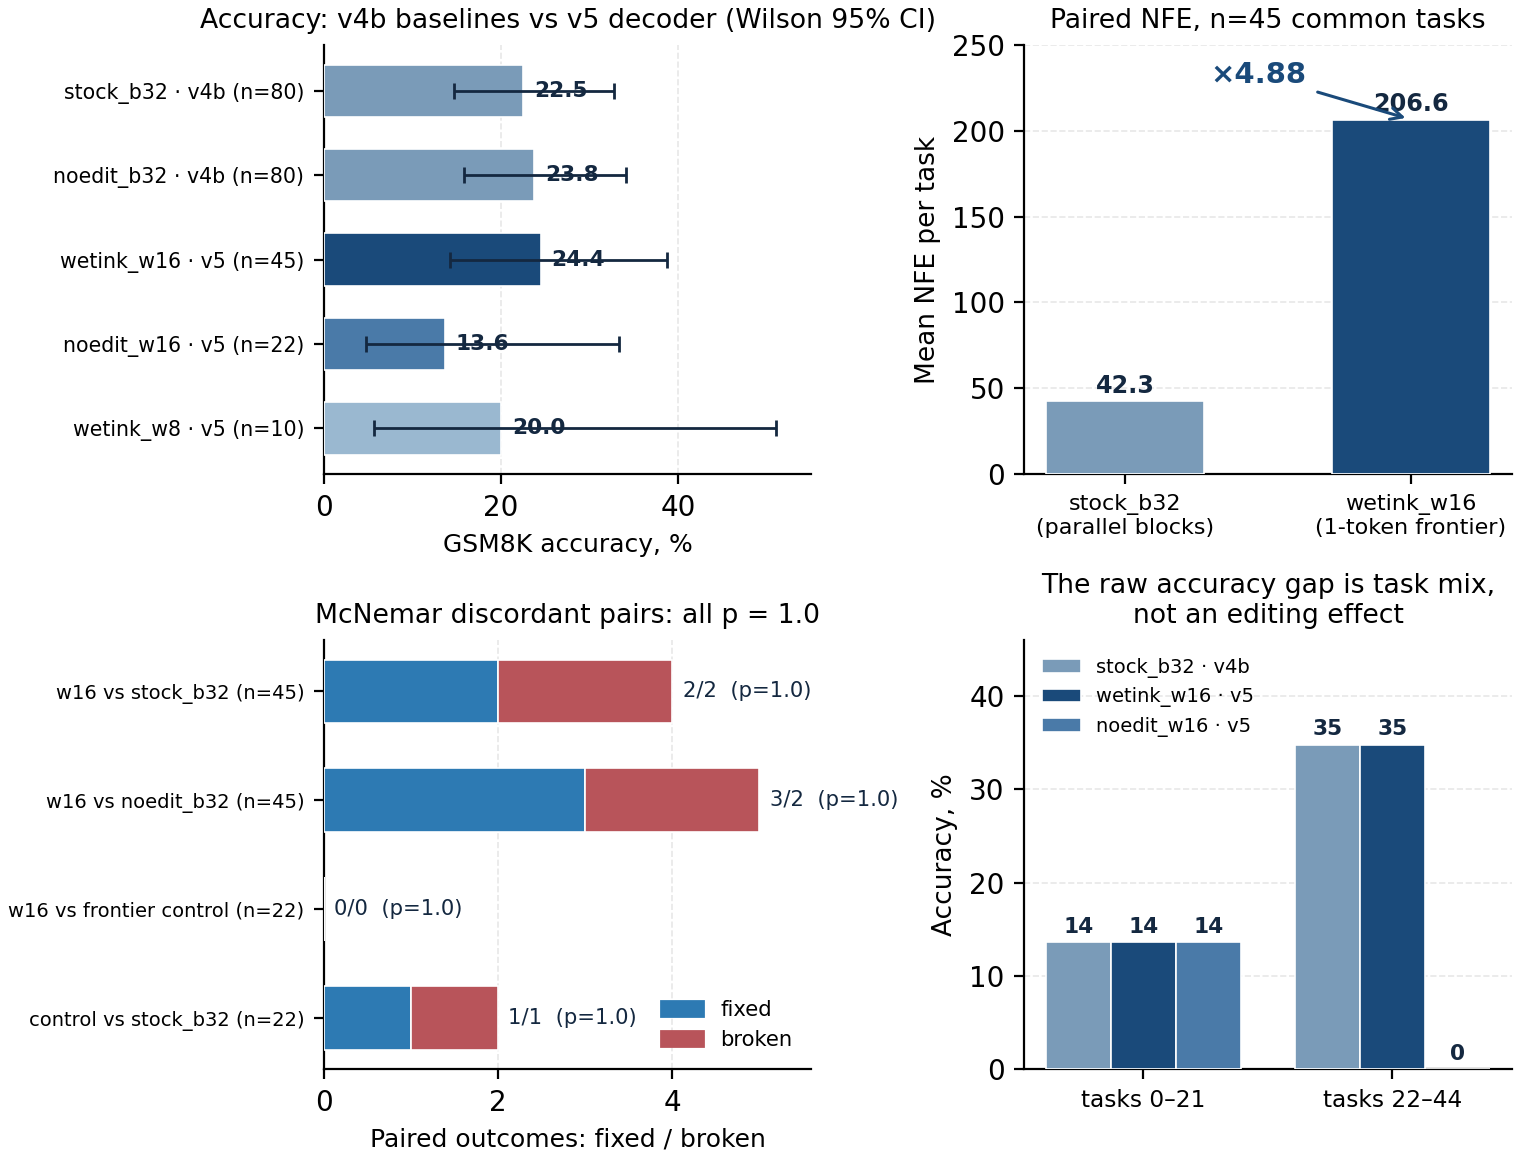
\includegraphics[width=0.96\textwidth]{fig_results.png}
  \caption{\textbf{Results.} (a) Accuracy with Wilson 95\% intervals for all arms.
  (b) Paired NFE on common tasks: stock versus wet-ink ($\times 4.88$). (c) McNemar
  discordant pairs for four comparisons~--- all $p{=}1.0$. (d) Segment analysis:
  on the hard tasks 0--21 every arm scores 13.6\%; the raw accuracy gap between
  arms reflects which segments they cover, not an editing effect.}
  \label{fig:results}
\end{figure}

\subsection{Paired exact analysis}
Table~\ref{tab:paired} gives the paired outcomes. Against the stock baseline, the
wet-ink arm solves exactly the same number of the 45 common tasks (11 versus 11),
with 2 outcomes fixed and 2 broken (exact McNemar $p{=}1.0$). Against the
frontier-only control on the 22 common tasks, the window edits flip \emph{zero}
outcomes ($3/22$ versus $3/22$, $0$ fixed, $0$ broken). The control itself matches
the stock baseline ($3/22$ versus $3/22$, $p{=}1.0$). In other words: the
one-token frontier costs nothing in accuracy relative to stock decoding, and the
editing window adds nothing on top of the frontier.

\begin{table}[t]
\centering\small
\caption{Paired exact McNemar on common task indices. `Fixed' = solved by the
second arm only; `broken' = solved by the first arm only.}\label{tab:paired}
\begin{tabular*}{\textwidth}{@{\extracolsep{\fill}} l c c c c c}
\toprule
Comparison (common $n$) & Score A & Score B & Fixed & Broken & $p$ \\
\midrule
wetink\_w16 vs stock\_b32 (45)    & 11/45 & 11/45 & 2 & 2 & 1.0 \\
wetink\_w16 vs noedit\_b32 (45)   & 11/45 & 10/45 & 3 & 2 & 1.0 \\
wetink\_w16 vs control (22)       & 3/22  & 3/22  & 0 & 0 & 1.0 \\
control vs stock\_b32 (22)        & 3/22  & 3/22  & 1 & 1 & 1.0 \\
\bottomrule
\end{tabular*}
\end{table}

\subsection{The task-composition artifact}\label{sec:artifact}
The $+10.8$-point raw gap between the wet-ink arm ($24.4\%$) and its own
frontier-only control ($13.6\%$) deserves a careful look, because it is exactly
the kind of number that is usually reported as a win. The mechanism is mundane:
the control arm exhausted its time budget after the first 22 tasks, and the first
22 GSM8K indices are systematically harder for this model~--- under 4-bit
quantization and a 160-token cap~--- than indices 22--44. On the hard segment
(tasks 0--21) \emph{every} arm scores exactly $13.6\%$: stock, control, and
wet-ink. On the easier segment the wet-ink arm scores $34.8\%$ and the stock
baseline $25.9\%$. The raw gap is therefore a statement about which tasks each
arm happened to cover, not about editing; the paired tests, which compare only
common indices, correctly report no effect. We flag this because unpaired
comparisons between unequally-truncated arms are easy to make in budget-limited
GPU settings and would have produced a false positive here.

\subsection{NFE accounting and mechanics}
The wet-ink arms cost $206.6$ NFE per task versus $42.3$ for stock on the same 45
tasks~--- a structural $\times 4.88$ multiplier, the price of committing one token
per forward pass. This multiplier is \emph{predictable} (it cannot churn: progress
is one mask per step by construction), unlike our v1 experience where a
training-free revision rule inflated NFE $9$--$13\times$ with
$\sim$589 re-masking events per block, $\sim$0.4 of which were real changes. In v5
the trained gate fires 6.9 real rewrites per task (churn 5.6)~--- the editing
machinery is demonstrably active, not disabled~--- and yet moves no outcomes.
Mechanics were verified on all 77 generations: bit-exact $W{=}0$ equivalence
(\texttt{ids\_equal=True}, NFE $97{=}97$), zero residual special tokens, and
deterministic outputs under $T{=}0$.

\subsection{Five versions as an ablation narrative}\label{sec:journey}
Table~\ref{tab:journey} summarizes the program that led here. Read as one
experiment, it is a five-step attack on the same hypothesis: \emph{can inference-time
token revision improve a fixed dLLM?} Training-free rules on the fixed Nemotron
model were harmful (v2--v3); the trained stock gate with a fixed block window is
neutral (v4); the trained gate with the sliding window it was arguably designed
for is still neutral (v5). Three independent, paired, consistently null results
--- in line with the calibration of \citet{remeval}~--- shift the burden of proof
toward approaches that change training, not decoding.

\begin{table}[t]
\centering\small
\caption{The five-version program. v1--v3 used
Nemotron-Labs-Diffusion-3B; v4--v5 use LLaDA2.2-mini. Paired statistics where
arm sizes permit.}\label{tab:journey}
\begin{tabularx}{\textwidth}{l l X}
\toprule
Ver. & Decoding scheme & Outcome (paired) \\
\midrule
v1 & confidence-gate re-masking each stock step & $+$6 pts GSM8K but
$\times 9$--$13$ NFE churn; termination invariant broken \\
v2 & full published revision cycles (RemeDi, CoDR) & termination restored;
RemeDi harmful at short blocks, CoDR near-neutral \\
v3 & full benchmark, $n{=}200$ GSM8K $+$ 164 HumanEval & RemeDi $-12.5$ to
$-31.5$ pts ($p{<}0.001$); CoDR neutral ($p{=}1.0$) \\
v4 & stock \texttt{generate()} parameter audit (12 arms, 403 gens.) & stock T2T
gate neutral ($p{=}1.0$), $-15\%$ NFE; window does not slide \\
v5 & \textbf{wet-ink: sliding window over trained gate} & \textbf{paired-identical
to stock ($p{=}1.0$) at $\times 4.88$ NFE} \\
\bottomrule
\end{tabularx}
\end{table}

% ===================== 6. Discussion =====================
\section{Discussion}\label{sec:discussion}

\paragraph{Why is the trained gate inert here?}
The T2T gate of LLaDA2.2 was trained, via L-EBPO, in a regime where editing
happens \emph{inside} the current block while parallel denoising is still
resolving it~--- its rewrites correct early sampling noise within a block that is
still being written. Our schedule relocates those rewrites to a window behind a
one-token frontier, a distribution the gate was never trained on; the model's
confidences behind the frontier are apparently already well calibrated~--- the
gate fires (6.9 rewrites per task) but its rewrites are almost always
confidence-neutral polish, not error repair. The result echoes the diagnosis of
\citet{remeval}: the bottleneck is the dLLM's ability to \emph{detect} its own
mistakes, not the schedule through which revisions are applied. A gate trained
with a sliding window~--- or any trained mistake detector~--- is the natural next
experiment, and our kernel is ready to host it.

\paragraph{What the negative result buys.}
First, a clean baseline: any future claim that sliding-window revision helps a
LLaDA2-class model must now beat an honestly-paired null, and our segment analysis
(Section~\ref{sec:artifact}) gives reviewers a concrete failure mode~--- unequal
arm coverage~--- to check for. Second, a cost bound: the revision opportunity is
available at a predictable $\times 4.88$ NFE, and a $k$-token frontier would
divide that multiplier by $k$ without touching a single formula; if a future
trained gate does help, the engineering path to it is already cheap. Third, the
zero-invention methodology itself: every component of our decoder is verbatim
model code with runtime equivalence checks, which is what made the null result
interpretable rather than confounded by an accidental model change.

% ===================== 7. Limitations =====================
\section{Limitations}\label{sec:limitations}

Our conclusions are bounded by four constraints. (i) \emph{Sample size}: the main
arm has $n{=}45$ and the control $n{=}22$; Wilson intervals span $\pm 12$ points,
so we can exclude large effects but not effects of a few points; detecting a
$\pm 5$-point effect would require $n \geq 500$ per arm. (ii) \emph{One model,
one benchmark, one regime}: results are for LLaDA2.2-mini at 4-bit quantization
on GSM8K with greedy decoding and a 160-token cap that truncates most
generations; the HumanEval arm was skipped by the time budget. (iii)
\emph{Window sizes}: only $W{=}16$ (main) and $W{=}8$ (ablation, $n{=}10$) ran;
$W{=}32$ was not reached. (iv) \emph{Ablation identity}: the frontier-only
control differs from the wet-ink arm by the editing gate alone, but the wet-ink
family as a whole differs from stock decoding by the schedule; we disentangle
schedule cost (NFE) from editing effect (outcome flips), not the joint
interaction with sampling temperature, which we fixed at zero.

% ===================== 8. Conclusion =====================
\section{Conclusion}\label{sec:conclusion}

We implemented wet-ink decoding~--- a one-token left-to-right frontier with a
sliding window of revisable tokens and a hard dry edge~--- for a modern diffusion
language model, under a zero-invention policy in which every mechanism is the
base model's own trained code. Under a paired exact protocol the method preserves
the stock decoder's accuracy arm for arm (McNemar $p{=}1.0$ everywhere), its
apparent advantage over an internal control dissolves into a task-composition
artifact, and its cost is a predictable $\times 4.88$ NFE. Together with the four
earlier versions of this program, the evidence indicates that inference-time
token revision, by any rule so far published, does not improve a fixed diffusion
language model in the greedy, short-block regime; revision that helps will likely
have to be trained. Code, data, full telemetry, and the reproduction kernel are
public.\footnote{\url{https://github.com/Asilbekov/Explore} and
\url{https://huggingface.co/Freedomform/wet-ink-v5}}


% ===================== References =====================
\begin{thebibliography}{20}\small

\bibitem{llada}
S.~Nie, F.~Zhu, Z.~You, X.~Zhang, J.~Ou, J.~Hu, J.~Zhou, Y.~Lin, J.-R. Wen, and
C.~Li.
\newblock Large language diffusion models.
\newblock In \emph{Advances in Neural Information Processing Systems (NeurIPS)}, 2025.
\newblock arXiv:2502.09992.

\bibitem{llada22mini}
inclusionAI.
\newblock LLaDA2.2-mini: a lightweight agentic MoE diffusion language model with
Levenshtein editing.
\newblock Hugging Face model card, 2026.
\newblock \url{https://huggingface.co/inclusionAI/LLaDA2.2-mini}.

\bibitem{llada21}
T.~Bie, M.~Cao, X.~Cao, B.~Chen, F.~Chen, K.~Chen, et~al.
\newblock LLaDA2.1: speeding up text diffusion via token editing.
\newblock arXiv preprint arXiv:2602.08676, 2026.

\bibitem{dream7b}
J.~Ye, Z.~Xie, L.~Zheng, J.~Gao, Z.~Wu, X.~Jiang, Z.~Li, and L.~Kong.
\newblock Dream 7B: diffusion large language models.
\newblock arXiv preprint arXiv:2508.15487, 2025.

\bibitem{bd3lm}
M.~Arriola, A.~Gokaslan, J.~T. Chiu, Z.~Yang, Z.~Qi, J.~Han, S.~S. Sahoo, and
V.~Kuleshov.
\newblock Block diffusion: interpolating between autoregressive and diffusion language
models.
\newblock In \emph{International Conference on Learning Representations (ICLR), Oral}, 2025.
\newblock arXiv:2503.09573.

\bibitem{setdiffusion}
M.~Arriola, A.~Gokaslan, J.~T. Chiu, Z.~Yang, Z.~Qi, J.~Han, S.~S. Sahoo, and
V.~Kuleshov.
\newblock Set diffusion: interpolating token orderings between autoregression and
diffusion for fast and flexible decoding.
\newblock In \emph{International Conference on Machine Learning (ICML)}, 2026.
\newblock arXiv:2607.01775.

\bibitem{levt}
J.~Gu, C.~Wang, and J.~Zhao.
\newblock Levenshtein transformer.
\newblock In \emph{Advances in Neural Information Processing Systems (NeurIPS)}, 2019.
\newblock arXiv:1905.11006.

\bibitem{remeval}
S.~Frkovi\'c, M.~Jazbec, D.~Zhang, C.~A. Naesseth, I.~Bogunovic, and
E.~Nalisnick.
\newblock Re-evaluating confidence remasking in masked diffusion language models.
\newblock In \emph{Advances in Neural Information Processing Systems (NeurIPS)}, 2026.
\newblock arXiv:2606.12232.

\bibitem{remedi}
Z.~Huang, Y.~Wang, Z.~Chen, and G.-J. Qi.
\newblock Don't settle too early: self-reflective remasking for diffusion language
models.
\newblock arXiv preprint arXiv:2509.23653, 2025.

\bibitem{codr}
Y.~Wu, Q.~Zhang, Y.~Zhang, and J.~Huang.
\newblock CoDR: training-free confidence-drift remasking for diffusion language
models.
\newblock arXiv preprint arXiv:2610.08833, 2026.

\bibitem{fastdllm}
C.~Wu, H.~Zhang, S.~Xue, Z.~Liu, S.~Diao, L.~Zhu, P.~Luo, S.~Han, and E.~Xie.
\newblock Fast-dLLM: training-free fast diffusion large language model inference.
\newblock arXiv preprint arXiv:2505.22618, 2025.

\bibitem{apd}
D.~Israel, G.~Van~den~Broeck, and A.~Grover.
\newblock Accelerating diffusion LLMs via adaptive parallel decoding.
\newblock arXiv preprint arXiv:2506.00413, 2025.

\bibitem{jys}
Y.-H. Park, C.-H. Lai, S.~Hayakawa, Y.~Takida, and Y.~Mitsufuji.
\newblock Jump your steps: optimizing sampling schedule of discrete diffusion models.
\newblock arXiv preprint arXiv:2410.07761, 2024.

\bibitem{proseco}
Y.~Schiff, O.~Belhasin, R.~Uziel, G.~Wang, M.~Arriola, G.~Turok, R.~Zilberstein,
M.~Elad, and V.~Kuleshov.
\newblock Learn from your mistakes: self-correcting masked diffusion models.
\newblock arXiv preprint arXiv:2602.11590, 2026.

\bibitem{saber}
Y.~Dong, Z.~Ma, X.~Jiang, et~al.
\newblock Saber: an efficient sampling with adaptive acceleration and backtracking
enhanced remasking for diffusion language models.
\newblock arXiv preprint arXiv:2510.18165, 2025.

\end{thebibliography}

\end{document}
